% Fragmento de entrega (sin preambulo; se compila desde main.tex).
\section*{Problema 2 -- Teoría de kernels circulares}

Sea $t$ un ángulo en el círculo, con periodo $2\pi$, y sean $P_1=24$ y
$P_2=7$ los periodos de la hora y del día de semana. La distancia circular
$d(t,t')$ es el arco más corto entre ambos puntos, con valores en $[0,\pi]$:
si $\Delta=|t-t'|\pmod{2\pi}$ es el recorrido en un sentido, entonces
$d=\min(\Delta,2\pi-\Delta)$.

\subsection*{(a) La distancia circular y el mapa del coseno}

Por definición, $d(23{:}00,01{:}00)=\frac{2\pi\cdot 2}{24}=\frac{\pi}{6}\approx 0.524$:
de las 23:00 a la 1:00 hay 2 horas de recorrido en un sentido
($\Delta=2\cdot(2\pi/24)$) y $2\pi-\Delta$ en el otro, y el arco más corto es
$2\cdot(2\pi/24)=\pi/6$; en cambio la diferencia de los números es $|23-1|=22$.
Análogamente, con sábado $=6$ y lunes $=1$ en $P=7$,
$\Delta=|6-1|\cdot(2\pi/7)=5\cdot(2\pi/7)$ y $2\pi-\Delta=2\cdot(2\pi/7)$, de
modo que $d(\text{sábado},\text{lunes})=2\cdot\frac{2\pi}{7}=\frac{4\pi}{7}\approx 1.795$
(dos días de distancia, aunque los números difieren en $5$).

Sea $\varphi(t)=(\cos t,\sin t)$. Entonces $\|\varphi(t)\|^2=1$ y
\[
\|\varphi(t)-\varphi(t')\|^2
=\|\varphi(t)\|^2+\|\varphi(t')\|^2-2\,\varphi(t)\cdot\varphi(t')
=2-2\cos(t-t'),
\]
porque $\varphi(t)\cdot\varphi(t')=\cos t\cos t'+\sin t\sin t'=\cos(t-t')$
y $\cos$ es par y $2\pi$-periódica, de modo que $\cos(t-t')=\cos d$ con $d$
el arco más corto. La función $2-2\cos d$ es estrictamente creciente en
$[0,\pi]$ porque su derivada es $2\sin d>0$ en $(0,\pi)$. Por eso la cuerda y
el arco ordenan igual a los pares de puntos: si un par está más cerca que otro
con una medida, también lo está con la otra.

\begin{center}
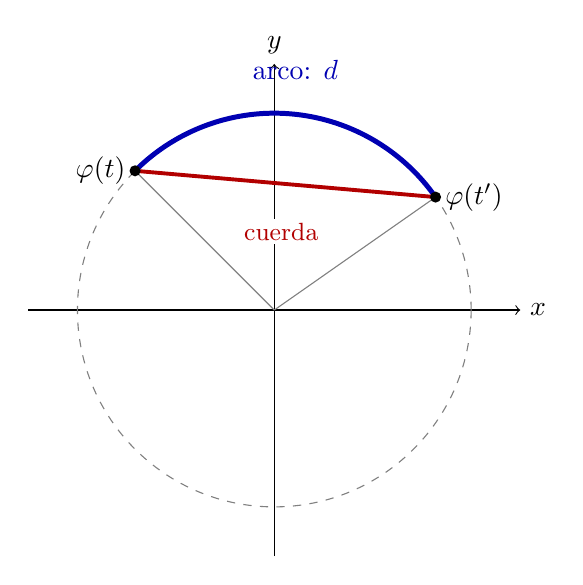
\begin{tikzpicture}[scale=1.25]
\draw[->] (-2.5,0) -- (2.5,0) node[right]{$x$};
\draw[->] (0,-2.5) -- (0,2.5) node[above]{$y$};
\draw[gray,dashed] (0,0) circle (2);
\coordinate (A) at (135:2);
\coordinate (B) at (35:2);
\draw[gray] (0,0) -- (A);
\draw[gray] (0,0) -- (B);
\draw[line width=1.8pt,blue!70!black] (35:2) arc (35:135:2);
\draw[line width=1.4pt,red!70!black] (A) -- (B);
\fill (A) circle (1.6pt);
\fill (B) circle (1.6pt);
\node[left] at (A) {$\varphi(t)$};
\node[right] at (B) {$\varphi(t')$};
\node[blue!70!black] at (85:2.45) {arco: $d$};
\node[red!70!black,fill=white,inner sep=1.5pt] at (85:0.8) {\small cuerda};
\end{tikzpicture}
\end{center}

El arco azul mide $d$ (el ángulo, en el círculo unitario) y la cuerda roja mide
$\|\varphi(t)-\varphi(t')\|=\sqrt{2-2\cos d}$, que es una función creciente de
$d$.

\subsection*{(b) El kernel de von Mises es un kernel}

Un kernel gaussiano sobre $\varphi$ es
$\exp\bigl(-\|\varphi(t)-\varphi(t')\|^2/(2\sigma^2)\bigr)
=\exp\bigl(-(2-2\cos(t-t'))/(2\sigma^2)\bigr)
=e^{-1/\sigma^2}\,e^{\cos(t-t')/\sigma^2}$,
es decir, $k_\kappa(t,t')=e^{\kappa\cos(t-t')}$ multiplicado por la constante
$e^{-\kappa}>0$, con $\kappa=1/\sigma^2$.

Por el inciso (a), $\cos(t-t')=\varphi(t)\cdot\varphi(t')$ es un kernel, con
función de características $\varphi=(\cos,\sin)$. Expandimos la exponencial en
serie de Taylor,
\[
e^{\kappa\cos(t-t')}
=\sum_{m=0}^{\infty}\frac{\kappa^m}{m!}\bigl(\cos(t-t')\bigr)^m,
\]
y aplicamos (P1): cada potencia $\cos^m(t-t')$ es un producto de kernels, así
que es un kernel; multiplicarla por $\kappa^m/m!>0$ lo conserva, las sumas
parciales son kernels, y el límite puntual de una sucesión de kernels es un
kernel. Por tanto $e^{\kappa\cos(t-t')}$ es un kernel y, multiplicado por
$e^{-\kappa}>0$, $k_\kappa$ también \textbf{es} un kernel.

\subsection*{(c) Por qué funciona el criterio de Fourier}

\textbf{La mitad fácil de (P2).} Supongamos $k(t,t')=g(t-t')=a_0+\sum_{n\ge1}a_n\cos(n(t-t'))$
con $a_n\ge0$ para todo $n$. Como
$\cos(n\theta-n\theta')=\cos(n\theta)\cos(n\theta')+\sin(n\theta)\sin(n\theta')$,
cada sumando $a_n\cos(n(t-t'))$ es el producto interno
$\varphi_n(t)\cdot\varphi_n(t')$ con $\varphi_n(t)=\sqrt{a_n}\,(\cos nt,\sin nt)$,
y el término constante $a_0$ es el kernel de $\varphi_0(t)=\sqrt{a_0}$. Así,
cada sumando es un kernel, las sumas parciales lo son por (P1), y el límite
puntual de las sumas parciales (la serie de Fourier de $g$, que converge a $g$
al ser continua) también lo es por (P1). Luego $k$ es un kernel.

\textbf{La otra mitad (cómo la usaría).} Si algún $a_n<0$, entonces $k$
\textbf{no} es un kernel, y hay que exhibir un vector que lo muestre. Se toma el
conjunto equiespaciado $t_i=2\pi i/N$, $i=0,\dots,N-1$, con $0<n<N/2$, y el
vector $v_i=\cos(nt_i)$. Usando
$\cos(m(t_i-t_j))=\cos(mt_i)\cos(mt_j)+\sin(mt_i)\sin(mt_j)$,
\[
v^{T}Kv=a_0\Bigl(\sum_i v_i\Bigr)^2+\sum_{m\ge1}a_m\Bigl[\Bigl(\sum_i v_i\cos(mt_i)\Bigr)^2+\Bigl(\sum_i v_i\sin(mt_i)\Bigr)^2\Bigr].
\]
Para $0<n<N/2$ se cumple $\sum_i v_i=0$, $\sum_i v_i\sin(mt_i)=0$ para todo $m$
y $\sum_i v_i\cos(mt_i)=N/2$ si $m\equiv\pm n \pmod N$ y $0$ en otro caso.
Por tanto
\[
v^{T}Kv=\frac{N^{2}}{4}\sum_{\substack{m\ge1\\ m\equiv\pm n\,(\mathrm{mod}\ N)}}a_m
=\frac{N^{2}}{4}\bigl(a_n+a_{N-n}+a_{N+n}+a_{2N-n}+\cdots\bigr).
\]
Los coeficientes distintos de $a_n$ son sus \emph{alias} en la malla de $N$
puntos. Como $g$ es continua y suave a trozos, $\sum_m|a_m|<\infty$, así que
los alias tienden a $0$ cuando $N$ crece; entonces, si $a_n<0$, para $N$
suficientemente grande $v^TKv<0$ y $k$ no es un kernel. Con una malla pequeña
los alias pueden compensar a $a_n$, y esto explica lo que ocurre con $k_I$ en
siete puntos (inciso (d)).

\subsection*{(d) Ningún candidato es un kernel}

Con $g(t)=k(d=|t|)$ sobre $[-\pi,\pi]$, los coeficientes de Fourier
$a_n=\frac{2}{\pi}\int_0^\pi g(t)\cos nt\,dt$ ($n\ge1$) tienen forma cerrada.
Para $k_I=e^{-d^2/2}$ (completando el cuadrado en la integral),
\[
a_n^{(I)}=\sqrt{\tfrac{2}{\pi}}\;e^{-n^2/2}\;\operatorname{Re}\,\operatorname{erf}\!\Bigl(\tfrac{\pi-in}{\sqrt2}\Bigr).
\]
Para $k_{II}=\max(0,1-d^2/4)$, que se anula para $d\ge2$, integrando por partes,
\[
a_0^{(II)}=\frac{4}{3\pi},\qquad
a_n^{(II)}=\frac{2}{\pi}\Bigl[-\frac{\cos 2n}{n^{2}}+\frac{\sin 2n}{2n^{3}}\Bigr]\quad(n\ge1).
\]
Estas fórmulas coinciden con la cuadratura numérica de la libreta 01
(primeros 40 coeficientes y gráficas):

\begin{itemize}
\item \textbf{$k_I=\exp(-d^2/2)$ \textbf{no} es un kernel.} El primer
coeficiente negativo es $a_4\approx-3.19\times10^{-4}$ (también son negativos
$a_6,a_8,\dots$, todos los pares). Contraejemplo: las 24 horas
$t_i=2\pi i/24$ y el vector $v_i=\cos(2\pi\cdot4\,i/24)$, $i=0,\dots,23$ (con
$n=4$). La computadora da $v^{T}Kv\approx-0.0583$ con $v^{T}v=12$; el menor
valor propio de la matriz de las 24 horas es $\lambda_{\min}\approx-0.00505$.
En el inciso (c), $\frac{N^2}{4}a_4=144\,a_4\approx-0.0459$ es el término
dominante, y el valor exacto incluye sus alias $a_{20},a_{28},\dots$.

\item \textbf{$k_{II}=\max(0,1-d^2/4)$ \textbf{no} es un kernel.} El primer
coeficiente negativo es $a_3\approx-0.0712$ (hay más negativos: $a_6,a_7,a_9,\dots$).
Contraejemplo: las 24 horas y $v_i=\cos(2\pi\cdot3\,i/24)$ (con $n=3$), que da
$v^{T}Kv\approx-10.07$ con $v^{T}v=12$ ($144\,a_3\approx-10.25$ más alias) y
$\lambda_{\min}\approx-0.839$.
\end{itemize}

\textbf{Un conjunto de puntos que engaña.} Con los \textbf{siete días}
($t_i=2\pi i/7$), la matriz de $k_I$ \emph{sí} resulta semidefinida positiva,
con $\lambda_{\min}\approx+0.0326>0$. Es una matriz circulante y su valor
propio de frecuencia $3$ es $\frac{7}{2}(a_3+a_4+a_{10}+a_{11}+\cdots)$: el
coeficiente negativo $a_4\approx-3.19\times10^{-4}$ cae como alias sobre
$a_3\approx+0.00966$, que lo domina. Esto \textbf{no contradice} nada: la
definición de kernel exige que $K$ sea semidefinida positiva para
\textbf{todos} los conjuntos finitos de puntos, y basta uno que falle (las 24
horas) para que $k_I$ no lo sea; que un conjunto concreto no revele el
problema es compatible con que no lo sea. Para $k_{II}$ los siete días sí lo
revelan ($\lambda_{\min}\approx-0.197$). Por eso en la práctica (M4) se usan
kernels circulares válidos y no estos candidatos.

\subsection*{(e) Varias variables a la vez: suma y producto}

Sean $k_1$ en las horas y $k_2$ en las temperaturas, con funciones de
características $\phi_1$ y $\phi_2$.

\begin{itemize}
\item \textbf{Suma.} Con $\phi_+(h,t)=(\phi_1(h),\phi_2(t))$ (concatenación),
\[
\phi_+(h,t)\cdot\phi_+(h',t')=\phi_1(h)\cdot\phi_1(h')+\phi_2(t)\cdot\phi_2(t')
=k_1(h,h')+k_2(t,t')=k_+\bigl((h,t),(h',t')\bigr),
\]
así que $k_+$ es un kernel. La SVM predice
$f(h,t)=\sum_i\alpha_i\,k_+\bigl((h_i,t_i),(h,t)\bigr)+b
=\underbrace{\sum_i\alpha_i k_1(h_i,h)}_{f_1(h)}+\underbrace{\sum_i\alpha_i k_2(t_i,t)}_{f_2(t)}+b$.
Es \textbf{aditiva}: el efecto de la hora, $f_1(h)$, no depende de la
temperatura.

\item \textbf{Producto.} Con $\phi_\times(h,t)=\phi_1(h)\otimes\phi_2(t)$ se
tiene $\langle\phi_1\otimes\phi_2,\phi_1'\otimes\phi_2'\rangle=
\langle\phi_1,\phi_1'\rangle\langle\phi_2,\phi_2'\rangle=k_\times$, consistente
con (P1). Ahora
$f(h,t)=\sum_i\alpha_i\,k_1(h_i,h)\,k_2(t_i,t)+b$:
el peso que recibe cada $k_1(h_i,h)$ es $\alpha_i k_2(t_i,t)$, que depende de
$t$. Por tanto \textbf{sí hay interacción}: el efecto de la hora puede cambiar
con la temperatura.
\end{itemize}

Por eso la estructura elegida en la práctica,
$(k_{hr}\cdot k_{wd})+k_{rbf}$, impone interacción entre hora y día de la
semana (el patrón horario de los días laborales difiere del de los fines de
semana) y deja un efecto aditivo para las demás variables estandarizadas.
